\section{Full Prompt Level Specifications}
\label{app:prompts}

\subsection{Classification}
\begin{enumerate}
  \item Bare text input only.
  \item Add task label: ``Classify the sentiment of the following text as
    Positive, Negative, or Neutral.''
  \item Add format constraint: ``Respond with only the single label word.''
  \item Add label definitions: Positive = expresses approval or satisfaction;
    Negative = expresses dissatisfaction or criticism; Neutral = neither or mixed.
  \item Add persona: ``You are an expert sentiment analyst.''
  \item Add guidelines: rules for ironic text, mixed sentiment, and domain jargon.
  \item Add worked example: a complete input/output example with explanation.
\end{enumerate}

\subsection{Product Extraction}
\begin{enumerate}
  \item Bare product listing text only.
  \item List required output fields: name, price, brand, category.
  \item Specify JSON output format with exact key names.
  \item Define each field: name = product title, price = numeric value without
    currency symbol, brand = manufacturer name, category = product type.
  \item Add persona (expert product data analyst) and missing-field instruction
    (use null for absent fields).
  \item Add extraction guidelines for ambiguous cases: implied brand names,
    price ranges, composite product names.
  \item Add full worked example: verbose product description with correct JSON output.
\end{enumerate}

\subsection{Question Answering}
\begin{enumerate}
  \item Question only.
  \item Add task label: ``Answer the following question.''
  \item Add format guidance: ``Be concise and direct.''
  \item Add domain context appropriate to the question.
  \item Add expert persona.
  \item Add uncertainty instruction: express uncertainty explicitly if unsure.
  \item Add worked example.
\end{enumerate}

\subsection{Math Reasoning}
\begin{enumerate}
  \item Problem statement only.
  \item Add task label: ``Solve the following math problem.''
  \item Add answer format: ``Give a single numeric answer.''
  \item Add show-work instruction: ``Show your reasoning step by step.''
  \item Add math tutor persona.
  \item Add step-by-step guidelines and common error warnings.
  \item Add worked example with full solution.
\end{enumerate}

\subsection{Summarisation}
\begin{enumerate}
  \item Article text only.
  \item Add task label: ``Summarise the following article.''
  \item Add length target: ``Write a summary of approximately 50--80 words.''
  \item Add content guidance: include who, what, when, where.
  \item Add journalist persona.
  \item Add quality guidelines: avoid redundancy, preserve key facts.
  \item Add worked example: article with reference summary.
\end{enumerate}

\subsection{Instruction Following}
\begin{enumerate}
  \item Topic prompt only (``List benefits of exercise'').
  \item Add task label and constraints explicitly stated.
  \item Add format specification mirroring the constraint type.
  \item Add constraint definitions (e.g., bullet = ``-'' or ``*'' prefix).
  \item Add writing expert persona.
  \item Add formatting guidelines and error examples.
  \item Add worked example satisfying all constraints.
\end{enumerate}

\section{LLM Judge Rubric}
\label{app:judge}

All responses are scored by the primary judge (\texttt{gpt-4o-mini}) and
the second judge (\texttt{gemini-2.0-flash}) using the following prompt
template.
The \texttt{\{rubric\}} placeholder is filled with a task-specific rubric
(Table~\ref{tab:rubrics}).

\begin{quote}
\small
\ttfamily
You are an expert judge evaluating an AI assistant's response.\\[4pt]
Task type: \{task\_type\}\\
Evaluation guidance: \{rubric\}\\
Reference answer (if available): \{ground\_truth\}\\[4pt]
AI response to evaluate:\\
\{response\}\\[4pt]
Rate the response on these 4 dimensions, each from 1 (very poor) to 5
(excellent):\\
- correctness: Does the response accurately answer the task?\\
- completeness: Is the response complete and thorough?\\
- reasoning: Is the reasoning or logic sound and clear?\\
- conciseness: Is the response appropriately concise?\\[4pt]
Respond ONLY with valid JSON in this exact format:\\
\{"correctness": <1-5>, "completeness": <1-5>, "reasoning": <1-5>,
"conciseness": <1-5>\}
\end{quote}

\begin{table}[h]
\centering
\caption{Task-specific rubrics provided to both LLM judges.}
\label{tab:rubrics}
\small
\begin{tabular}{lp{10cm}}
\toprule
Task & Rubric \\
\midrule
Classification &
  Focus on Correctness (does the classification match the reference label?).
  Conciseness rewards direct labelling without padding.
  Reasoning Quality assesses any justification given.
  Completeness checks if the classification is unambiguous. \\
\addlinespace
Product Extraction &
  Focus on Correctness (do the extracted fields match the reference values?).
  Completeness checks if all 4 fields (name, price, brand, category) are present.
  Reasoning Quality is less relevant; focus on extraction accuracy.
  Conciseness rewards clean JSON output without extra text. \\
\addlinespace
QA &
  Focus heavily on Correctness (does the answer match the reference?).
  Completeness checks if the answer is fully given.
  Reasoning Quality assesses logical justification.
  Conciseness penalises unnecessary verbosity. \\
\addlinespace
Math Reasoning &
  Focus on Correctness (does the final numerical answer match the reference?).
  Completeness checks if work is shown.
  Reasoning Quality assesses whether the solution steps are logical.
  Conciseness penalises unnecessary verbosity beyond the solution. \\
\addlinespace
Summarisation &
  Focus on Completeness (coverage of key points from the reference).
  Correctness checks factual accuracy.
  Conciseness rewards brevity over length.
  Reasoning Quality assesses coherence and structure. \\
\addlinespace
Instr.\ Following &
  Focus on Completeness (are all stated constraints satisfied?).
  Correctness checks format and structural adherence.
  Conciseness rewards appropriate brevity.
  Reasoning Quality assesses overall response clarity. \\
\bottomrule
\end{tabular}
\end{table}

\section{Per-Model Saturation Statistics}
\label{app:stats}

Table~\ref{tab:full-stats} reports fit type, R$^2$, F-test $p$-value, and
saturation token count for all 42 (model, task) pairs in the main study.

\begin{table}[h]
\centering
\caption{Complete saturation statistics for all model--task pairs.
  Bold: F-test $p < 0.05$.
  Fit = best-fit curve type (log = logarithmic, sig = sigmoid).}
\label{tab:full-stats}
\footnotesize
\begin{tabular}{llccrr}
\toprule
Model & Task & Fit & R$^2$ & $p$ & $T^*$ \\
\midrule
llama-3.1-8b  & QA                 & log & 0.291 & 0.503 & 43  \\
llama-3.1-8b  & Summarisation      & sig & 0.161 & 0.896 & 104 \\
llama-3.1-8b  & Classification     & sig & 0.866 & 0.079 & 75  \\
\textbf{llama-3.1-8b}  & \textbf{Instr.\ Following} & sig & \textbf{0.929} & \textbf{0.031} & \textbf{112} \\
llama-3.1-8b  & Math Reasoning     & sig & 0.125 & 0.928 & 81  \\
llama-3.1-8b  & Product Extraction & sig & 0.720 & 0.229 & 234 \\
\midrule
gemini-flash  & QA                 & sig & 0.404 & 0.622 & 8   \\
gemini-flash  & Summarisation      & sig & 0.760 & 0.185 & 69  \\
\textbf{gemini-flash}  & \textbf{Classification}    & sig & \textbf{0.936} & \textbf{0.027} & \textbf{42}  \\
gemini-flash  & Instr.\ Following  & log & 0.067 & 0.871 & 15  \\
gemini-flash  & Math Reasoning     & sig & 0.205 & 0.853 & 51  \\
gemini-flash  & Product Extraction & sig & 0.830 & 0.113 & 471 \\
\midrule
qwen3-32b     & QA                 & log & 0.690 & 0.096 & 20  \\
qwen3-32b     & Summarisation      & sig & 0.106 & 0.944 & 83  \\
qwen3-32b     & Classification     & log & 0.753 & 0.061 & 164 \\
qwen3-32b     & Instr.\ Following  & sig & 0.465 & 0.544 & 27  \\
qwen3-32b     & Math Reasoning     & sig & 0.217 & 0.840 & 63  \\
\textbf{qwen3-32b}     & \textbf{Product Extraction} & log & \textbf{0.930} & \textbf{0.005} & \textbf{378} \\
\midrule
llama-3.3-70b & QA                 & log & 0.065 & 0.875 & 43  \\
llama-3.3-70b & Summarisation      & log & 0.290 & 0.503 & 104 \\
\textbf{llama-3.3-70b} & \textbf{Classification}    & sig & \textbf{0.957} & \textbf{0.015} & \textbf{64}  \\
llama-3.3-70b & Instr.\ Following  & log & 0.379 & 0.385 & 50  \\
llama-3.3-70b & Math Reasoning     & sig & 0.282 & 0.769 & 84  \\
\textbf{llama-3.3-70b} & \textbf{Product Extraction} & sig & \textbf{0.943} & \textbf{0.023} & \textbf{92}  \\
\midrule
kimi-k2       & QA                 & log & 0.097 & 0.816 & 34  \\
kimi-k2       & Summarisation      & log & 0.664 & 0.113 & 95  \\
\textbf{kimi-k2}       & \textbf{Classification}    & sig & \textbf{0.955} & \textbf{0.016} & \textbf{57}  \\
kimi-k2       & Instr.\ Following  & log & 0.027 & 0.947 & 41  \\
kimi-k2       & Math Reasoning     & sig & 0.339 & 0.702 & 74  \\
kimi-k2       & Product Extraction & log & 0.695 & 0.093 & 342 \\
\midrule
gpt-4o-mini   & QA                 & log & 0.646 & 0.125 & 15  \\
gpt-4o-mini   & Summarisation      & log & 0.356 & 0.414 & 76  \\
\textbf{gpt-4o-mini}   & \textbf{Classification}    & sig & \textbf{0.977} & \textbf{0.006} & \textbf{50}  \\
gpt-4o-mini   & Instr.\ Following  & log & 0.386 & 0.377 & 22  \\
gpt-4o-mini   & Math Reasoning     & sig & 0.178 & 0.879 & 54  \\
gpt-4o-mini   & Product Extraction & sig & 0.877 & 0.071 & 422 \\
\midrule
claude-haiku  & QA                 & log & 0.618 & 0.146 & 15  \\
\textbf{claude-haiku}  & \textbf{Summarisation}     & log & \textbf{0.824} & \textbf{0.031} & \textbf{83}  \\
claude-haiku  & Classification     & sig & 0.646 & 0.317 & 38  \\
claude-haiku  & Instr.\ Following  & log & 0.071 & 0.863 & 23  \\
claude-haiku  & Math Reasoning     & sig & 0.228 & 0.829 & 60  \\
\textbf{claude-haiku}  & \textbf{Product Extraction} & sig & \textbf{0.980} & \textbf{0.005} & \textbf{536} \\
\bottomrule
\end{tabular}
\end{table}

\section{Qualitative Examples}
\label{app:examples}

\paragraph{Classification (gpt-4o-mini, ``Absolutely love this laptop...'').}
\begin{itemize}
  \item \textbf{L1} (30 tokens, $q=0.90$): ``This review can be classified as
    \textbf{Positive}.''---correct label embedded in verbose explanation.
  \item \textbf{L3} (44 tokens, $q=1.00$): ``Positive''---just the label,
    higher quality because format matches.
  \item \textbf{L7} (182 tokens, $q=1.00$): ``positive''---no further
    improvement despite 6$\times$ more prompt tokens.
\end{itemize}

\paragraph{Product extraction (gemini-flash, ``Nike Air Max 270...'').}
\begin{itemize}
  \item \textbf{L1} (37 tokens, $q=0.70$): Bulleted list with extra
    fields---correct information but wrong format.
  \item \textbf{L3} (63 tokens, $q=0.80$): JSON with correct fields, but
    ``Air Max 270'' instead of ``Nike Air Max 270'' for name.
  \item \textbf{L7} (271 tokens, $q=1.00$):
    \texttt{\{"name": "Nike Air Max 270", "price": "150", "brand": "Nike",
    "category": "shoes"\}}---the worked example teaches the exact output
    schema.
\end{itemize}

\section{Output Length Control}
\label{app:output}

Output length varies across levels. We computed partial correlations
controlling for output length to confirm the prompt$\to$quality relationship
is not an artefact of output compression.

\begin{table}[h]
\centering
\caption{Partial correlations controlling for output length.}
\label{tab:partial}
\small
\begin{tabular}{lrr}
\toprule
Task & $r$(output, quality) & partial $r$(prompt, quality $|$ output) \\
\midrule
Classification      & $-0.186$ & $0.106$ \\
Product extraction  & $-0.313$ & $0.447$ \\
Instr.\ following   & $0.616$  & $0.209$ \\
\bottomrule
\end{tabular}
\end{table}

The prompt$\to$quality relationship persists after controlling for output
length (positive partial $r$ for all three tasks).

\section{Replication Experiment}
\label{app:replication}

% TODO: Include replication figures
% \begin{figure}[h]
%   \centering
%   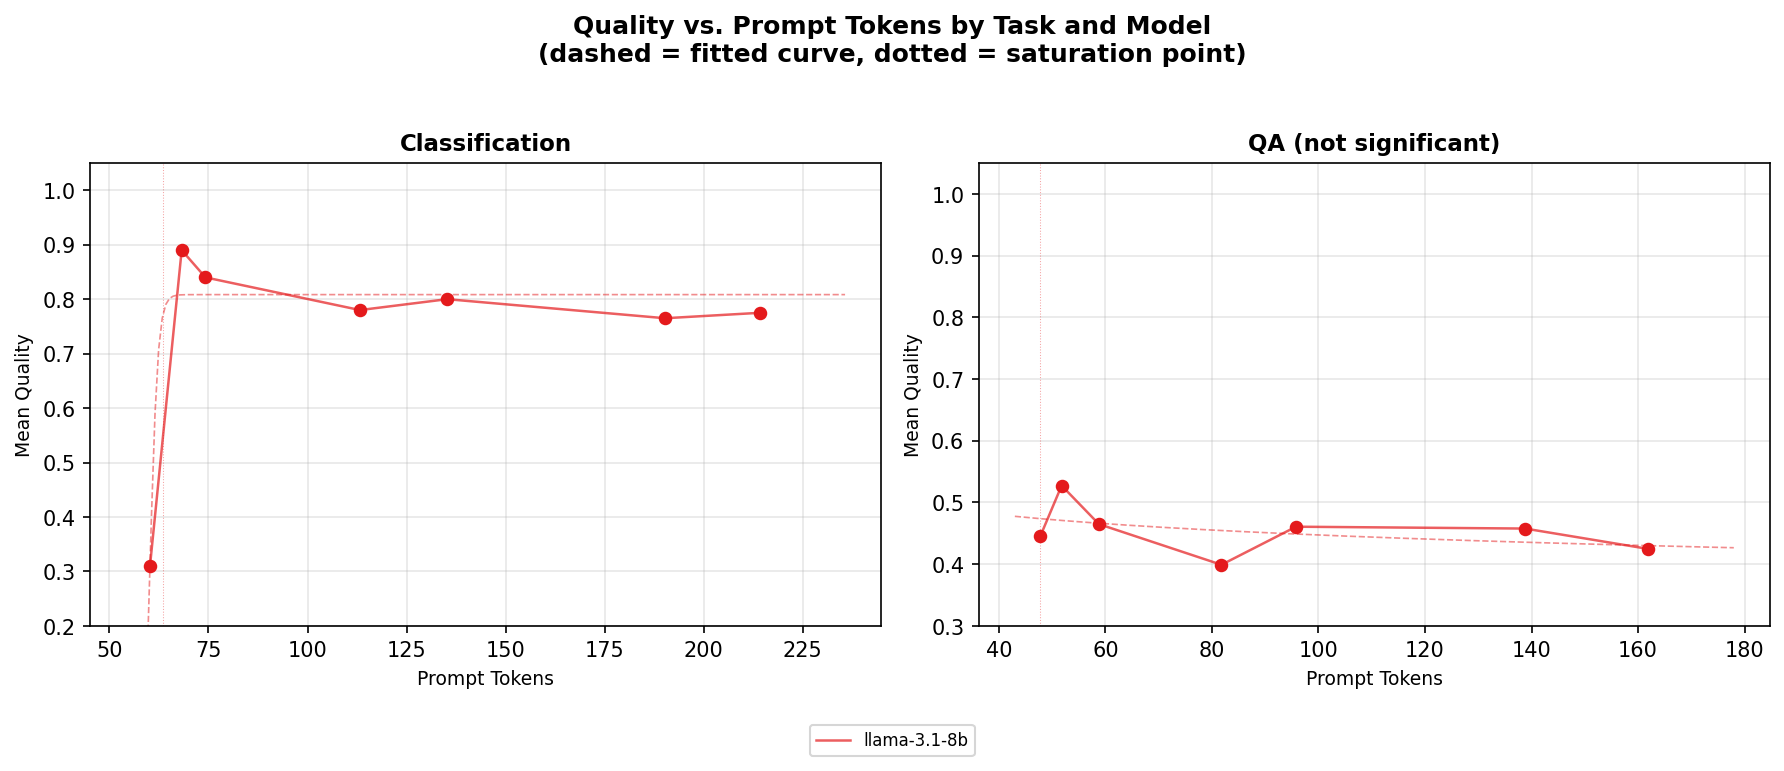
\includegraphics[width=\linewidth]{figures/fig_replication_curves.png}
%   \caption{200-example replication: classification shows clear saturation;
%     QA shows no systematic improvement.}
%   \label{fig:replication}
% \end{figure}

The 200-example replication on SST-2 (classification) and SQuAD (QA)
confirms the main-study findings.
Classification saturates at approximately 64 tokens with a narrow bootstrap
CI, while QA shows no statistically significant relationship between prompt
length and quality.
